\section{Design}
Here we present the VAPP's structure and implementation details,
as well as the history and reasoning that led to this final approach.
Our design assumes a shared memory multiprocessor system and does
not require hardware support.

\subsection{VAPP Modules}
The three primary layers of VAPP are a
Pin\footnote{http://www.pintool.org/} tool for dynamic binary
instrumentation, a SQLite\footnote{http://www.sqlite.org/} database to
store application traces, and a collection of replay and analysis
programs. In addition, we have written two libraries that are used for
logging control and core replay functionality. These components and
their relationship is shown in Figure \ref{fig:overview}.

\begin{figure*}
  \begin{center}
  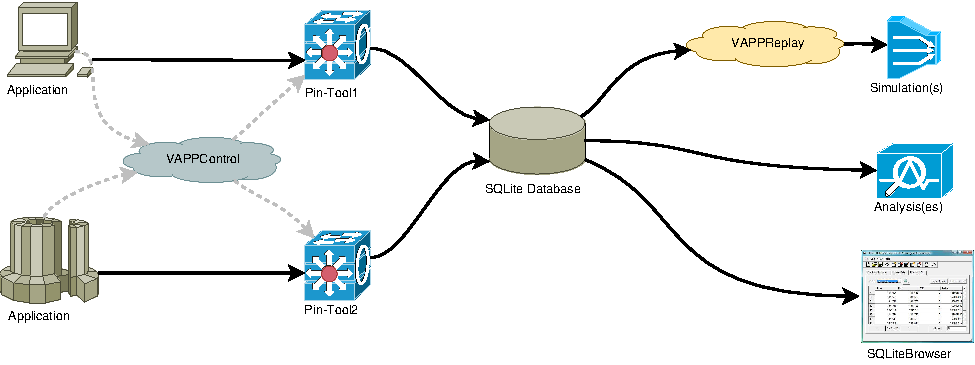
\includegraphics[width=.9\textwidth]{overview}
  \caption{Application of different platforms can be analyzed by any
    of our pin-tools. Using out VAPPControl library applications can
    limit the gather trace information in scope and time. Each
    pin-tool will write its data into a single sqlite database
    file. This database file will then be used as source for our
    analysis (SQL based or direct) and as input to out VAPPReplay
    library. The VAPPReplay library provides a simple C++ class
    abstract for the ease of developing analysis or simulations.}
  \label{fig:overview}
  \end{center}
\end{figure*}

\subsection{Pin Tool}
While Pin is very feature-rich in terms of the kinds of information
it provides access to during instrumented application execution, this
comes at a cost with regard to execution time.  Given that we wished to
design a tool that would allow programmers to repeatedly run and rerun
their applications on a large set of architecture configurations,
one design goal was to make this process as fast as possible.  We assume
that the application will be executed on very many types of simulated
architectures, and thus concluded that the best way to reduce the
total time to conduct the simulations would be to log an execution trace
and amortize the slowdown from the Pin tool over many replays.  Note that
this approach further assumes that the application designer wishes to
use the same set of input for all replays or sufficiently large
groups of replays.

To be precise, we have implemented two distinct Pin tools to focus
on the detailed logging required for application replay and the
different trace requirements needed for the analysis of parallel
program correctness respectively.  In theory, these two tools could
be merged and log the union of all data that each individual tool
tracks.  However, we discovered that from a practical standpoint
such an approach could be seriously inefficient, in particular
when the user desires some form of analysis that does not
require full application replay.  That is, in order to replay
application execution, it is necessary to log all memory accesses
an other information at a very detailed level.  However, our
analysis of parallel programs can be achieved with a much more
coarse execution trace and logging less results in faster execution
and perhaps more importantly much smaller logs.  Smaller log file in
turn lead to faster database accesses and faster execution of our
analysis programs.

As mentioned above, the replay-oriented pin tool must log memory
operations in great detail, which conflicts with our desire to
keep the log database as small as possible for performance reasons.
Therefore, our final design allows the application to dynamically
turn selectively switch certain subsets of the logging on and off
or entirely disable the trace some of the execution.  This is
achieved via simple calls to our VAPP control library, which 
only requires the application code to specify which logging
features are to be enabled or disabled at that point.
The Pin tool instruments such library calls and then adjust the
logging accordingly.  The specific trace information that can
be controlled in this manner is function calls, memory accesses,
memory allocations and deallocations, and locking and unlocking.

The parallel program-oriented tool is able to track execution
as a coarser grain by analyzing memory operations at the level
of buffers instead of individual addresses.  We define a buffer
as the block of memory that is allocated by a single call to
\texttt{malloc}.  Thus, all parallel program correctness analysis,
such as lockset analysis, is also performed at the level of buffers.
Consequently, programs that lock memory at finer level, for instance
by having different locks to protect different rows or blocks of a matrix,
can lead to false positives in the analysis routines.
Given the performance benefits, we feel that this is a reasonable tradeoff.

\subsection{Database Functionality and Schema}
We chose SQLite to store our application traces for its usability
and portability.  The entire database that stores the logs is
saved as a single file that can be easily moved across machines
or archived.  In addition, SQLite was easy to learn and begin
using, which was of critical importance given the strict timeline
for our project.  Moreover, the open source
SQLite Database Browser\footnote{http://sqlitebrowser.sourceforge.net/}
allows application programmers (our intended users) to easily view
and query the SQLite database, which was a significant goal of our
work.  By exposing the logged data, developers can implement
certain analysis and explore their application's behavior directly
without writing custom replay code.  Figures \ref{pic:sqlite_browse}
and \ref{pic:sqlite_query}
provide one such an example where a user is investigating
whether a particular memory buffer is accessed by a single thread.


\begin{figure}
  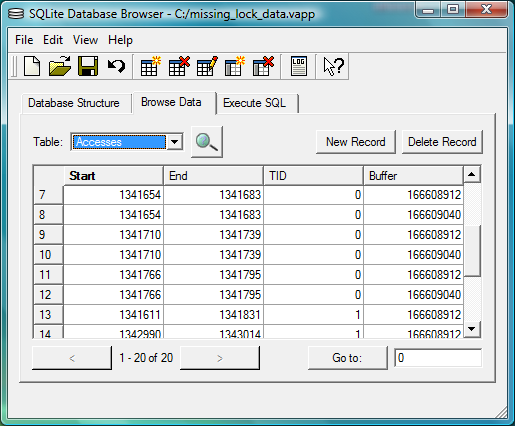
\includegraphics[width=\columnwidth]{sqlite_browse}
  \caption{Storing application traces as an SQLite database
  	allows users to easily access the data with the SQLite
  	Database Browser.}
  \label{pic:sqlite_browse}
\end{figure}


\begin{figure}
  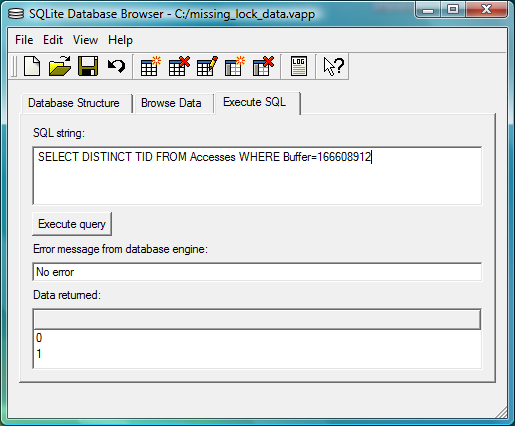
\includegraphics[width=\columnwidth]{sqlite_query}
  \caption{Users can query the SQLite database to learn
  	about their application's execution.  Here the user
  	has determined that a particular memory buffer was
  	accessed by multiple threads.}
  \label{pic:sqlite_query}
\end{figure}


Figure \ref{pic:db_schema1} shows the database schema for the first
Pin tool, that records all memory operations. The schema consists of
the following tables:
\begin{description}
  \item[Images] Tracks information about which images
    (i.e. executables and dynamic libraries) are used by the
    program). The table records the name (\texttt{ImgName}) of the
    image and an associated, unique numerical identifier
    (\texttt{Id}).
  \item[Calls] Records all methods calls performed during
    execution. An entry consists of the simulation time
    (\texttt{VLCK}) the event occurred, the memory base address
    (\texttt{Method}) of the method and the action (\texttt{Enter}),
    i.e. whether the program entered or left the method.
  \item[Methods] Contains all available methods during the execution
    of the program. An entry of this table consists of the Method name
    (\texttt{MethName}), the id (\texttt{ImgId}) of the image within
    which the method is located, the base address (\texttt{MethStart})
    at which the method is located in memory and the address of the
    last method instruction (\texttt{MethEnd}).
  \item[MemoryAccesses] Records all occurred memory accesses. If an
    instruction has more than one memory access (e.g., instruction and
    data access) then multiple entries are generated. An entry
    consists of the simulation time (\texttt{VLCK}) the event
    occurred, The memory address that is accesses
    (\texttt{MemAddress}), the address of the instruction that
    triggered the event (\texttt{InstrAddress}), an numerical value
    (\texttt{ThreadId}) specifying in which thread the event occurred
    and field identifying (\texttt{Write}) whether the operation was a
    read or write.
  \item[Frees] This table records all executed \texttt{free} calls. An
    entry in this table consists of the simulation time
    (\texttt{VLCK}) the call occurred and the base address
    (\texttt{Address}) of the buffer.
  \item[Mallocs] This table records all memory allocations via
    \texttt{malloc}. An entry in this table consists of the simulation
    time (\texttt{VLCK}) the call occurred, the size of the allocated
    buffer (\texttt{Size}) and the base address (\texttt{Address}) of
    the buffer.
\end{description}


\begin{figure}
  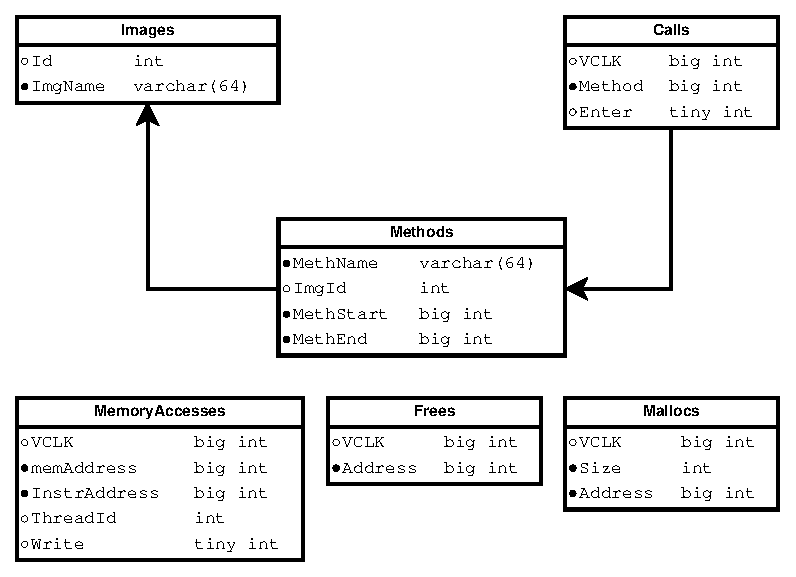
\includegraphics[width=\columnwidth]{database_schema1}
  \caption{Database Schema Pin-Tool1}
  \label{pic:db_schema1}
\end{figure}


Figure \ref{pic:db_schema2} illustrates the database
schema of the Pin tool designed for parallel program analysis.
The schema is composed of the the follow tables:
\begin{description}
  \item[Threads] This table gather all information of the threads that
    have been executed during the program execution. An entry in the
    table consists of the time the thread has been created
    (\texttt{Start}), the time the thread terminated (\texttt{End}) and
    an unique,numerical identifier (\texttt{TID}).
  \item[Accesses] This tables track execution epochs and the buffers
    touched during this execution period. To avoid a variable length
    entries in the database we use fixed size entries to specify one
    buffer/epoch mapping. An entry in this table consists of the time
    the execution epoch begins (\texttt{Start}), the time when it ends
    (\texttt{End}), the number of the thread that executed this epoch
    (\texttt{TID}) and the base address of the buffer
    (\texttt{Buffer}).
  \item[Locks] This table records all executed 
    \texttt{pthread\_mutex\_lock} and
    \texttt{GOMP\_critical\_start} calls. An entry in this table
    consists of the simulation time (\texttt{VLCK}) the call occurred,
    the base address (\texttt{Address}) of the lock and the
    numerical identifier of the thread performing the operation
    (\texttt{TID}).
  \item[UnLocks] This table records all executed
    \texttt{pthread\_mutex\_unlock} and
    \texttt{GOMP\_critical\_end} calls. An entry in this table
    consists of the simulation time (\texttt{VLCK}) the call occurred,
    the base address (\texttt{Address}) of the lock and the
    numerical identifier of the thread performing the operation
    (\texttt{TID}).
  \item[Frees] This table records all executed \texttt{free} calls. An
    entry in this table consists of the simulation time
    (\texttt{VLCK}) the call occurred, the base address
    (\texttt{Address}) of the buffer and the numerical identifier of
    the thread performing the operation (\texttt{TID}).
  \item[Mallocs] This table records all memory allocations via
    \texttt{malloc}. An entry in this table consists of the simulation
    time (\texttt{VLCK}) the call occurred, the size of the allocated
    buffer (\texttt{Size}), the base address (\texttt{Address}) of
    the buffer and the numerical identifier of
    the thread performing the operation (\texttt{TID}).
\end{description}

\begin{figure}
  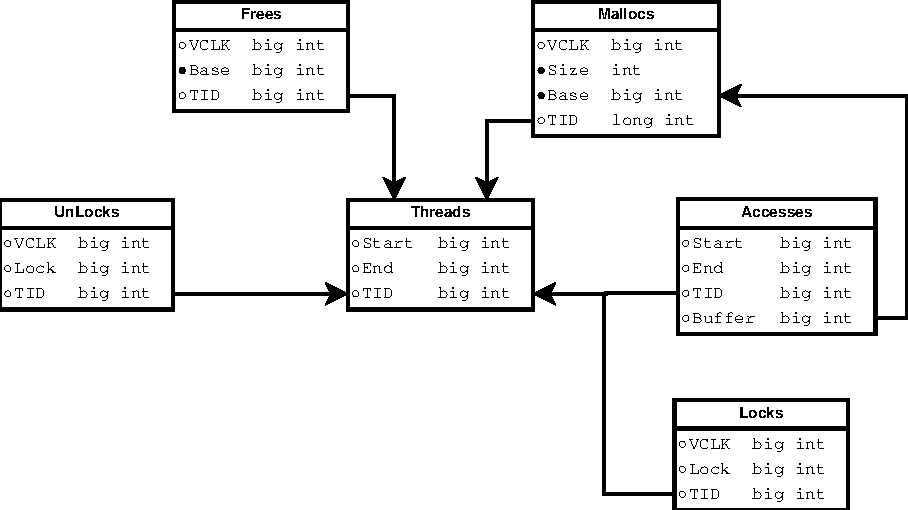
\includegraphics[width=\columnwidth]{database_schema2}
  \caption{Database Schema Pin-Tool2}
  \label{pic:db_schema2}
\end{figure}


\subsection{Application Replay}
Presently, VAPP supports the replay of memory operations with
particular focus on memory accesses and usage patterns.  This
level of replay is sufficient to allow a user to simulate
execution on a variety of memory-related hardware components.
We felt this was an important area to focus on first because
memory accesses can oftentimes be the major bottleneck in program
performance.  By replaying memory operations, a developer can
investigate how varying levels of cache or page tables, cache 
configurations, shared/private caches, shared/separate L1 instruction
and data cache, etc. impact performance.

The core replay functionality is implemented in the VAPP replay
library. One of the central parts if the library is the Executor class
(see Figure \ref{fig:executor}). The Executor class is an abstract
class that provides callback methods for every memory
operations. Every simulation/analysis need to inherit from the
Executor class and implement the callback methods. The programmer then
can register its implementation (or several implementations if
necessary or required) with the library and start the replay.  The
replay library loads memory operations from the database and replays
them into every executor that has been attached to it.



\begin{figure*}
  \lstset{
    language=C++,
    basicstyle=\small,
  }
  \begin{lstlisting}
class Executor {
 public:
  virtual ~Executor() {}

  // is called for instructions that read one memory location
  virtual void memRead(long ip, long addr, int size) = 0;

  // is called for instructions that read two memory location
  virtual void memRead(long ip, long addr1, long addr2, int size) = 0;

  // is called for instructions that write to memory
  virtual void memWrite(long ip, long addr, int size) = 0;

  // called for all other instructions
  virtual void instruction(long ip) = 0;

  // is called when the simulation ends to generate the final report
  virtual void doReport(std::ostream &os) = 0;
};
  \end{lstlisting}
  \caption{The abstract Executor class, that every simulation needs to
    sub-class in order to receive memory callbacks.}
  \label{fig:executor}
\end{figure*}

\subsection{Parallel Program Analysis}
\label{sec:ppa}
Our analysis of code running on parallel architectures is
not replay-based and thus does not require individual memory
accesses to be logged or loaded.  Specifically, VAPP can
examine shared memory protection and locking behavior via
the classic lockset algorithm \cite{savage1997eraser},
determine which memory buffers are accessed by which threads,
and report which buffers are allocated but not used or not freed.

The goal of this analysis is to allow the programmer to make
educated architecture-centered decisions.  For instance, if
it is discovered that certain memory buffers are consistently
accessed only by a single processor, that information can be
fed back to the system so that this memory is pinned to that
processor's cache so that communication overhead is reduced.
Information regarding lock usage and contention can be
used to determine what types of low-level locking mechanisms
might be best for the application given the performance, 
communication, and space tradeoffs in these mechanisms.
Lockset analysis is an fundamental component in the analysis
of parallel program correctness. By reporting which
memory buffers are not protected by a consistent set of locks
when they are accessed, the programmer can detect concurrency
bugs. Conversely, if it is discovered that a buffer is
protected by multiple locks, the programmer may realize that
certain locks are redundant and improve performance by eliminated
unneeded locks.

We extended this analysis into a second set of analysis tools that allow the
user to analyze locksets amongst several different threads. This analysis
reports which buffers are shared amongst which threads along with
their corresponding locking set.

While there are a number of parallel programming models in use today,
VAPP focuses on the popular Open MP\footnote{http://openmp.org/wp/} and
pthreads\footnote{https://computing.llnl.gov/tutorials/pthreads/}
approaches.  Pthread-based parallel programs typically protect memory
via explicit calls to \texttt{pthread\_mutex\_lock} and
\texttt{pthread\_mutex\_unlock}, thus VAPP tracks these calls.  Open MP
support comes in the form of logging the use of critical sections
pragmas and the memory they protect. If the Open MP implementation
would use the pthread functionality then we would already have
everything in place to analyze Open MP programs. Unfortunately
the Open MP implementation of GCC (called GOMP) does not use pthread
mutexes. After analyzing the source code of the corresponding runtime
library, we discovered that the implementation uses system level
locks. Fortunately the runtime implementation used a similar
abstraction. Every time a critical section is entered the
\texttt{GOMP\_critical\_start} method is called to lock a default
lock, and the \texttt{GOMP\_critical\_end} method is call when leaving
a critical section to unlock the default lock. We therefore thread
like the \texttt{pthread\_mutex\_lock} and
\texttt{pthread\_mutex\_unlock} functions. Because the GOMP function
always lock a default lock, there is no need to pass the lock explicitly
as parameter to the function. We therefore cannot detect the lock
address when those methods are called. Fortunately we do not need the
exact address, because the those functions will always lock/unlock the
same lock. We therefore replace the lock address in the case of GOMP
function call with a magic value (in our case 666) that is unlikely
to be used elsewhere.

\subsection{Evolution From Initial Design}
VAPP's focus has evolved since it's inception.  Initially, the
majority of our efforts were to focus on the goal of making
single-threaded applications' execution traces accessible via SQL
queries, because we felt this was the most unique component of our
proposed work.  We also intended the support efficient iterative
simulations as the current version of VAPP does.  However, after
helpful discussions with Dr. Mowry we came to the conclusion that this
scope alone was more interesting to a software engineering audience
than the architecture community.  Thus, we scaled back our work on the
rich analysis that could be expressed purely as SQL queries and added
our parallel architecture-oriented goals as a major component of VAPP.

As discussed previously, the size of the SQLite database logs became
problematic when logging detailed traces on larger applications.  This
led us to introduce the VAPP trace control library, which allows
developers to only trace the most interested portions of an
application, thereby reducing the log size.  In addition, we realized
that parallel programs often share data at a somewhat coarse level in
order to reduce communication overhead and that logging every
individual memory access may not be necessary for their analysis.
Thus, we split the Pin tool so that the tool for parallel analysis
could log less detailed information at the level of memory buffers.
This resulted in a massive reduction in log size, which improved the
performance of both the Pin tool and the analysis programs.

Lastly, early on we intended to only support pthreads for our parallel
analysis, but found that we had time after completing our 100\% goals
to extend VAPP to support OpenMP as well. Due to the popularity of
OpenMP, this makes VAPP attractive to a much larger community of
developers. 


